\section{Experimental Evaluation}
\label{results}

Our evaluation is organized around the two claim boundaries introduced in
Section~\ref{aegis}: (i) \projectname~detects realistic HPC agent-compromise
patterns on the deployed stack with low operational cost, and (ii) that
coverage comes from the intended combination of constraint checking,
signature augmentation, and cross-agent correlation rather than from a single
heuristic. We therefore separate \emph{real-path} experiments, which measure the
implemented \ebpf-based attestation pipeline on EPYC hardware, from
\emph{simulation-based controlled studies}, which evaluate broader attack
coverage, ablation, baseline comparison, and benign-workload behavior under the
same policy semantics. The real-path experiments use the deployed
\projectname~probe, collector, verifier, and policy logic; the controlled
studies reuse the same attack families and policy semantics but execute them in
a deterministic harness that exposes larger attack and workload matrices.

\subsection{Methodology}

We evaluate the deployed stack on an AMD EPYC 7713-based node (64 cores at
2.0\,GHz, 256\,MB shared L3, and 1536\,GB system memory) running Rocky Linux
9.6 with Linux kernel 5.14.0. This platform is representative of current HPC
compute nodes. The \ebpf-based attestation engine is compiled with
\texttt{clang} and performs kernel-side syscall interception, while the
verifier executes the full \projectname~policy pipeline including
behavioral-constraint checking, cross-agent correlation, and containment
decision generation.

Our evaluation separates \emph{real-path measurements} from
\emph{controlled security studies}. The real-path measurements exercise the
implemented probe, collector, and verifier stack on the EPYC platform to
measure direct probe overhead, end-to-end detection latency, and per-attack
behavior. Unless stated otherwise, real-path results use a 1\,s attestation
interval and report medians over three repetitions per attack.

The controlled studies use the same policy semantics and attack families, but
execute them in a deterministic harness that exposes larger attack, ablation,
and workload matrices than are convenient to stage on a single node. We use
this harness for complete attack coverage, specialized-component ablation, the
benign-workflow false-positive study, the scaling analysis, and the baseline
comparison. Controlled attack outcomes are deterministic for a given trace; for
baseline timing we analyze each trace ten times and report mean analysis time.
The benign suite covers six workflows and 42 benign actions, including
authorized multi-agent collaboration, budget-edge LLM reporting, and tool-heavy
post-processing.

\subsection{Real-Path Detection Results}

Figure~\ref{fig:attack-results} summarizes the real-path detection results.
\projectname~detects all four implemented attack classes in 3/3 trials and in
the first post-injection attestation cycle. At the default 1\,s attestation
interval, the median detection latency is 500.27\,ms for filesystem-mediated
injection, 500.13\,ms for co-location injection, 500.19\,ms for supply-chain
injection, and 500.19\,ms for coordinated exfiltration. These latencies are
approximately half of the attestation interval because the attacks are injected
midway through a bundle window. Median data emitted before detection is 68\,B,
50\,B, 519\,B, and 503\,B, respectively. Median verifier CPU overhead stays
below 0.055\% in all cases.

\begin{figure}[t]
  \centering
  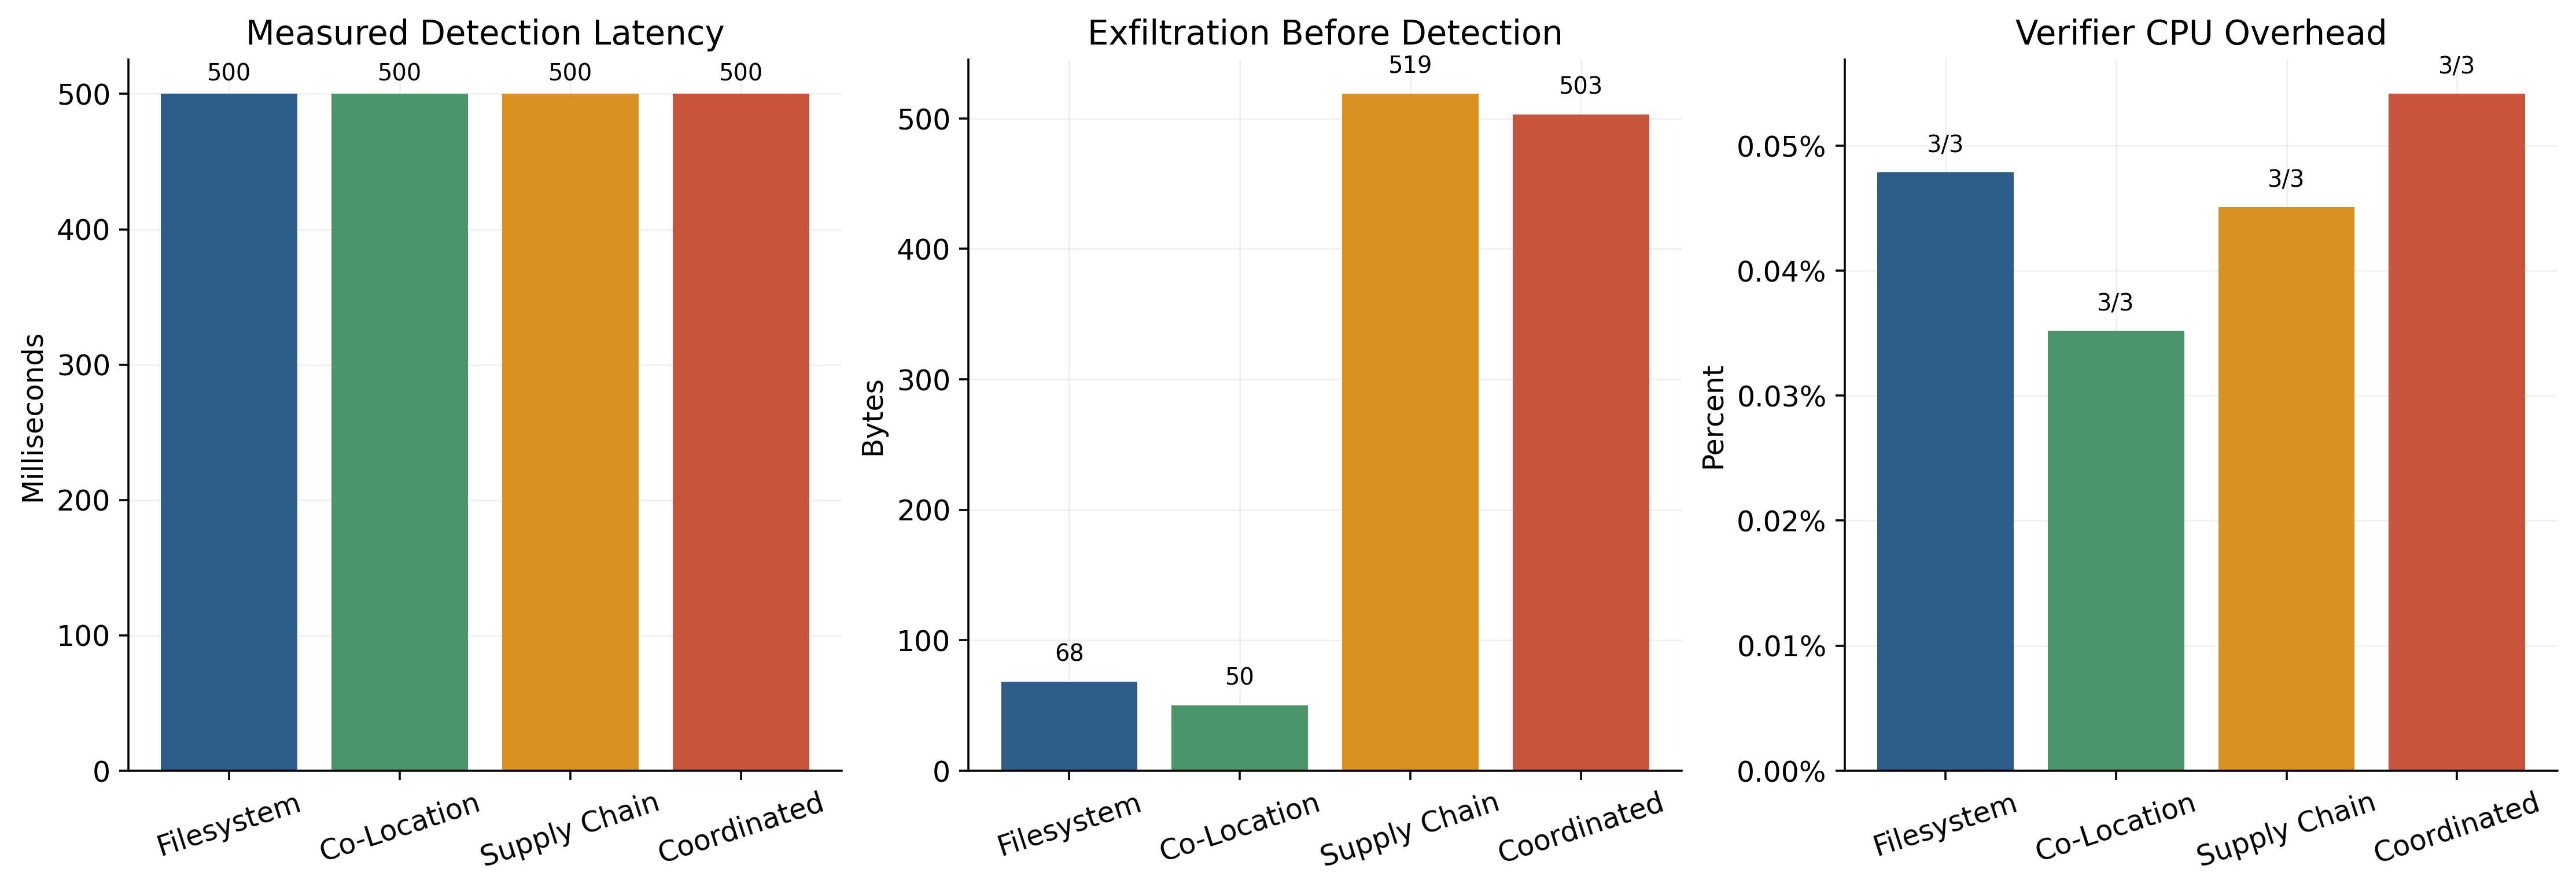
\includegraphics[width=\linewidth]{../figures/attack_results.png}
  \caption{Real-path outcomes at a 1\,s attestation interval. \projectname
  detects all four attacks in 3/3 trials with median detection latency of
  500.13--500.27\,ms and verifier CPU overhead below 0.055\%.}
  \label{fig:attack-results}
\end{figure}

Table~\ref{tab:real-path-summary} records the exact median values underlying
Figure~\ref{fig:attack-results}. The narrow latency spread across the four
real-path attacks indicates stable verifier behavior, while the emitted-byte
differences reflect attack semantics rather than detector instability.

\begin{table}[t]
  \caption{Exact real-path median measurements for the four implemented attacks at a 1\,s attestation interval.}
  \label{tab:real-path-summary}
  \centering
  \small
  \begin{tabular}{p{3.7cm}cccc}
    \toprule
    Attack & Trials & Latency (ms) & Exfil. (B) & CPU (\%) \\
    \midrule
    Filesystem injection & 3/3 & 500.27 & 68 & 0.0478 \\
    Co-location injection & 3/3 & 500.13 & 50 & 0.0352 \\
    Supply-chain injection & 3/3 & 500.19 & 519 & 0.0451 \\
    Coordinated exfiltration & 3/3 & 500.19 & 503 & 0.0542 \\
    \bottomrule
  \end{tabular}
\end{table}

The real-path results also show that \projectname~detects attacks through the
intended policy dimensions rather than through a single catch-all rule.
Filesystem injection triggers denied-path and unauthorized-endpoint violations,
co-location injection is detected through network policy, supply-chain
injection combines sensitive-file access with exfiltration policy, and
coordinated exfiltration triggers both denied-path violations and the
cross-agent covert-channel rule.

\subsection{Controlled Security Coverage}

To complement the real-path measurements, we run the full four-attack suite in
the controlled harness. Table~\ref{tab:controlled-coverage} summarizes these
results. In this setting, all four attacks succeed in hijacking the target
agent and exfiltrating data, and \projectname~detects all four, yielding a 100\%
detection rate over 4/4 completed attacks. The controlled suite produces 16
total findings and 1158\,B of exfiltrated payload across the four attacks. The
simpler filesystem and co-location attacks each trigger one detection, whereas
the supply-chain and coordinated attacks each trigger seven detections because
they violate multiple policy dimensions simultaneously. The coordinated attack
also raises an explicit covert-channel finding, confirming that the
cluster-wide access graph is necessary for this class of multi-agent attack.

\begin{table}[t]
  \caption{Controlled Security Coverage Across the Four Attack Classes}
  \label{tab:controlled-coverage}
  \centering
  \small
  \begin{tabular}{p{5.2cm}cccc}
    \toprule
    Attack & Detected & Findings & Time (ms) & Exfil. (B) \\
    \midrule
    Filesystem-mediated injection & Yes & 1 & 0.258 & 68 \\
    Multi-user co-location injection & Yes & 1 & 0.038 & 50 \\
    Supply-chain injection via skills & Yes & 7 & 0.089 & 519 \\
    Coordinated multi-agent exfiltration & Yes & 7 & 0.104 & 521 \\
    \bottomrule
  \end{tabular}
\end{table}

These controlled results matter for two reasons. First, they provide a fully
reproducible security-coverage view that is not tied to one hardware
configuration. Second, they show that the real-path detections are not
accidental: the same attack classes remain detectable when exercised in a
deterministic harness with the same policy semantics.

\subsection{Baseline Comparison}

Figure~\ref{fig:baseline-comparison} compares \projectname~against four
representative alternatives on the same deterministic attack traces. Network
DLP, filesystem auditing, and strict sandboxing each detect two of the four
attacks (50\%), while per-agent analytics misses all four. \projectname~is the
only defense that detects every attack class. The richer analysis does incur
higher processing cost than the simpler baselines, but the absolute cost
remains small: \projectname~averages 0.0614\,ms of analysis time per trace,
compared with 0.0038--0.0074\,ms for the baselines.

\begin{figure}[t]
  \centering
  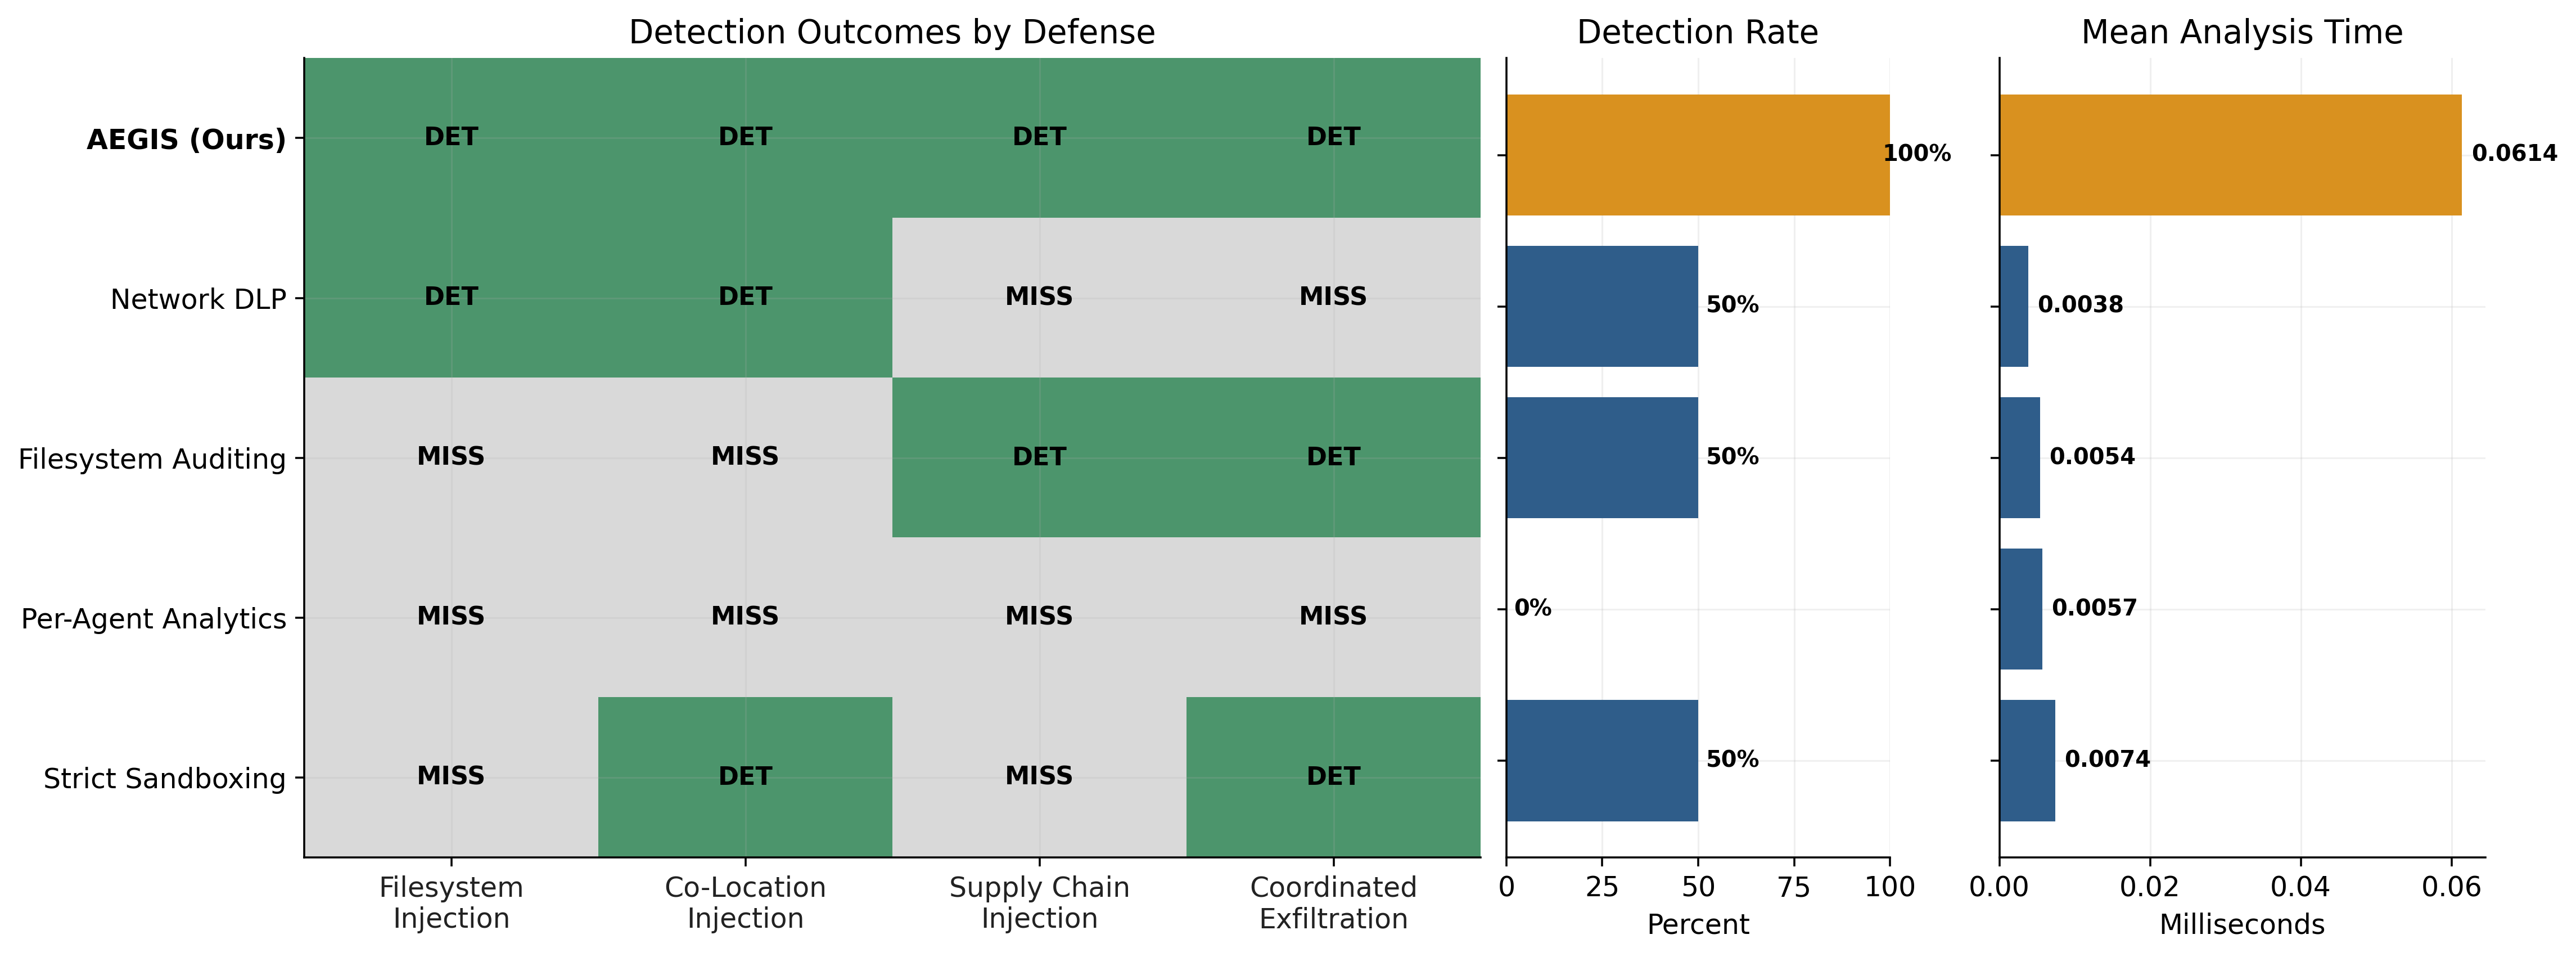
\includegraphics[width=\linewidth]{../figures/baseline_comparison.png}
  \caption{Baseline comparison on identical attack traces. \projectname~is the
  only defense that detects all four attacks; the simpler baselines detect at
  most two of four. Mean analysis time remains sub-0.1\,ms in all cases.}
  \label{fig:baseline-comparison}
\end{figure}

These results highlight why \projectname~needs all four policy dimensions. DLP
sees egress but cannot reason about encrypted traffic sent to whitelisted
services. Filesystem auditing sees sensitive paths but misses network-only
violations. Strict sandboxing blocks only the attacks that cross a hard
isolation boundary, and per-agent analytics misses coordinated behavior
entirely because the individual agents remain locally plausible. In contrast,
\projectname~combines constraint checking, signature augmentation, and
cross-agent correlation in a single verifier.

\subsection{Ablation}

The real-path ablation in Figure~\ref{fig:real-ablation} shows that measured
coverage comes from overlapping but non-identical mechanisms. Removing network
policy causes co-location injection to evade detection entirely (0/3), because
that attack is otherwise path-compliant. A permissive profile misses
filesystem, co-location, and supply-chain attacks in all three trials, but it
still detects coordinated exfiltration in all three trials because the
cluster-wide covert-channel rule remains active. In contrast, removing only
data-access controls, exfil-budget enforcement, or tool policy does not reduce
detection on this four-attack set, because the remaining active dimensions are
still sufficient. The real-path ablation therefore shows both redundancy and
specificity: several dimensions overlap, but network policy and cross-agent
correlation are indispensable for distinct attack classes.

\begin{figure}[t]
  \centering
  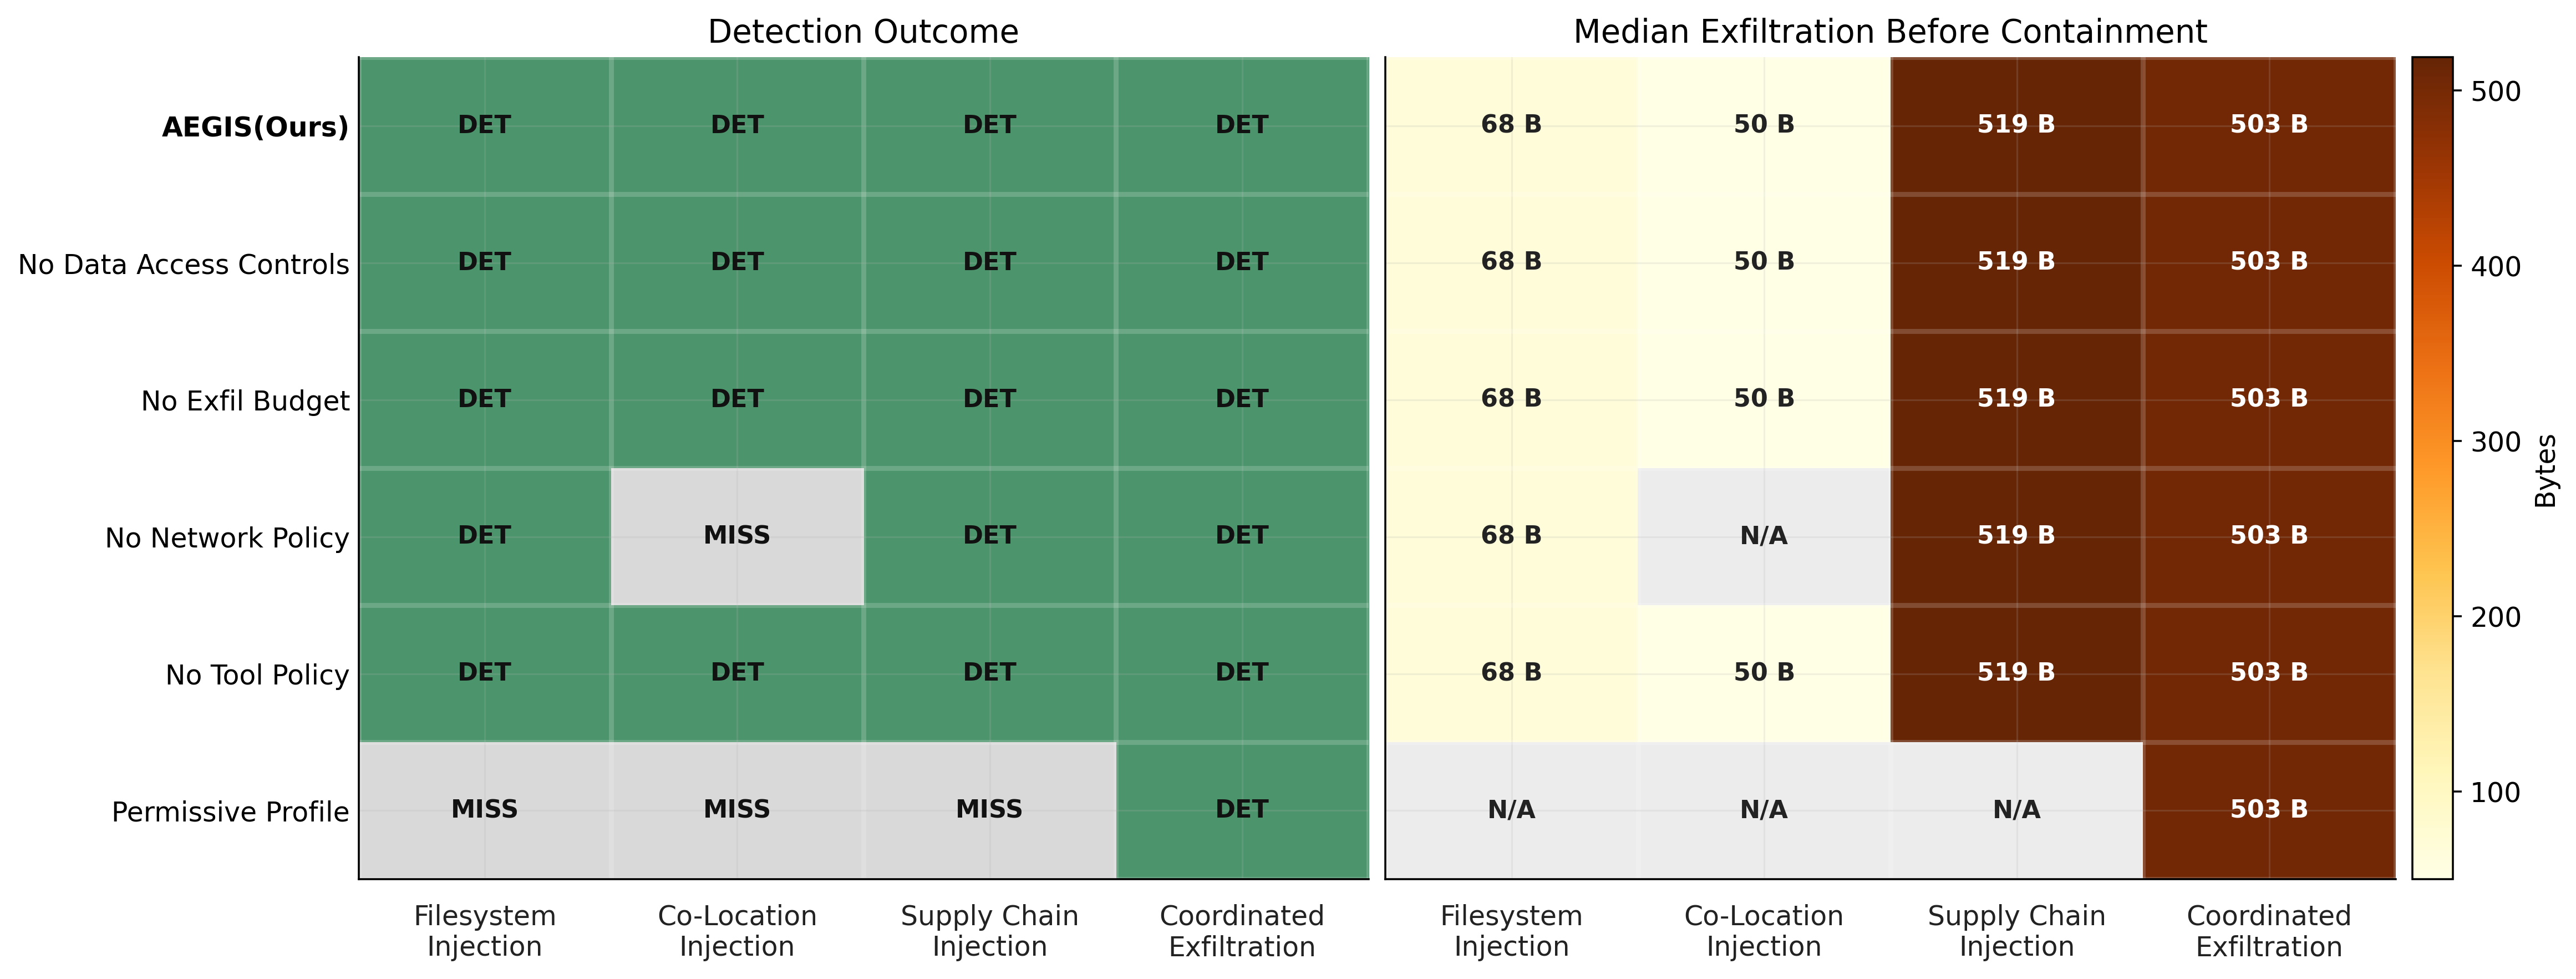
\includegraphics[width=\linewidth]{../figures/ablation_heatmap.png}
  \caption{Real-path ablation at a 1\,s attestation interval. Network policy
  is necessary for co-location injection, while the permissive profile misses
  all but coordinated exfiltration. The right panel reports median bytes
  emitted before containment.}
  \label{fig:real-ablation}
\end{figure}

Figure~\ref{fig:simulated-ablation} sharpens this observation by isolating the
specialized detection mechanisms more directly. In the simulation harness, full
\projectname~detects all four controlled attacks. Disabling egress-budget
enforcement, sensitive-file detection, covert-channel correlation, or injection
signatures drops detection from 100\% to 75\% by allowing exactly the
corresponding attack class to pass. A minimal path-only policy detects none of
the attacks. Taken together, the real and simulated ablations support the
intended interpretation: the constraint layer provides the primary security
boundary, while specialized checks add orthogonal coverage where generic path
constraints are insufficient.

\begin{figure}[t]
  \centering
  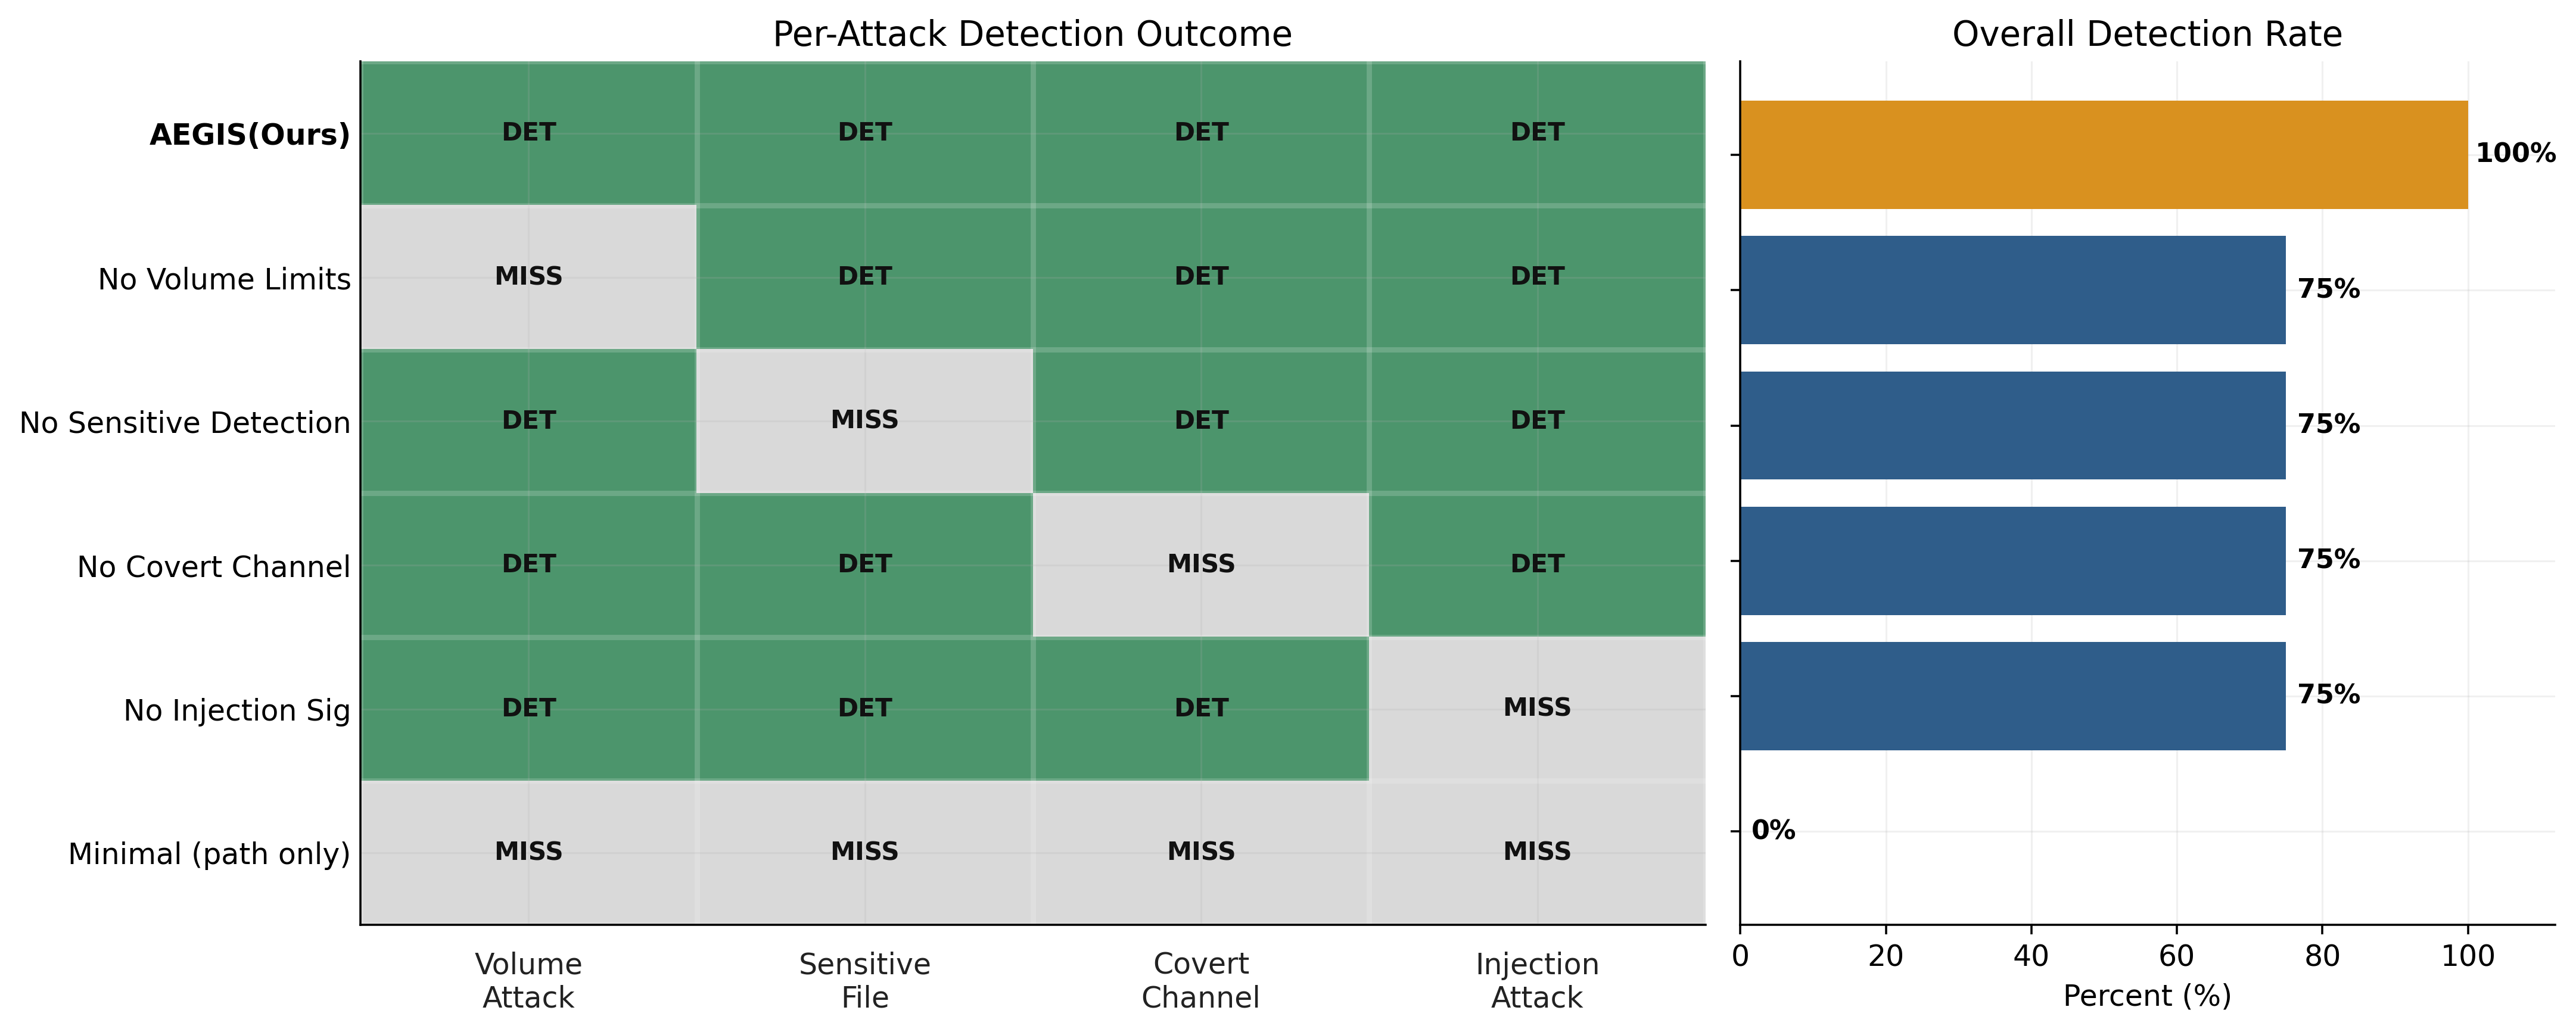
\includegraphics[width=\linewidth]{../figures/simulated_ablation_breakdown.png}
  \caption{Controlled ablation of specialized detection mechanisms. Removing
  any one mechanism drops detection from 100\% to 75\% by allowing its matching
  attack class to pass; a minimal path-only policy detects none.}
  \label{fig:simulated-ablation}
\end{figure}

\subsection{Performance}

Figure~\ref{fig:performance-overhead} combines the two most important
performance views. First, the direct probe microbenchmarks quantify worst-case
overhead when a single syscall family is exercised continuously. File-centric
syscalls are the most expensive: elapsed-time overhead is 24.0\% for
\texttt{openat} and 28.3\% for \texttt{read}, while network connection
monitoring adds 4.04\% for \texttt{connect}. These microbenchmarks are
deliberately pessimistic and should be interpreted as upper bounds on probe
cost rather than application-level slowdown. The same runs show throughput
losses of 19.4\% for \texttt{openat}, 22.1\% for \texttt{read}, and 3.9\% for
\texttt{connect}.

Second, the real end-to-end latency sweep shows that the operational overhead
of \projectname~on the full verifier path is substantially lower. All four
attacks remain detectable across the entire tested range from 100\,ms to
10\,s. Detection latency tracks the attestation interval, rising from 50.2\,ms
at a 100\,ms interval to 500.2\,ms at 1\,s and 5.00\,s at 10\,s. Over the
same interval sweep, verifier CPU overhead drops from 0.439\% to 0.039\% and
then to 0.0039\%. At the default 1\,s interval, which we use for the rest of
the real-path evaluation, the system therefore achieves sub-second detection
with approximately 0.04\% measured verifier CPU overhead.

Table~\ref{tab:interval-operating-points} lists the exact operating points
from this sweep and makes the deployment tradeoff explicit: the default 1\,s
setting sits near a practical knee of the curve, because moving to 500\,ms
roughly halves latency but nearly doubles verifier CPU cost, while relaxing to
2\,s halves CPU again but doubles detection latency.

\begin{table}[t]
  \caption{Real-path attestation-interval operating points from the latency sweep. All four attacks remain detectable at every tested interval.}
  \label{tab:interval-operating-points}
  \centering
  \small
  \begin{tabular}{cccc}
    \toprule
    Interval (s) & Avg. latency (ms) & CPU overhead (\%) & All detected \\
    \midrule
    0.1 & 50.17 & 0.4394 & Yes \\
    0.5 & 250.16 & 0.0767 & Yes \\
    \textbf{1.0 (default)} & \textbf{500.16} & \textbf{0.0392} & \textbf{Yes} \\
    2.0 & 1000.15 & 0.0208 & Yes \\
    5.0 & 2500.16 & 0.0080 & Yes \\
    10.0 & 5000.14 & 0.0039 & Yes \\
    \bottomrule
  \end{tabular}
\end{table}

\begin{figure}[t]
  \centering
  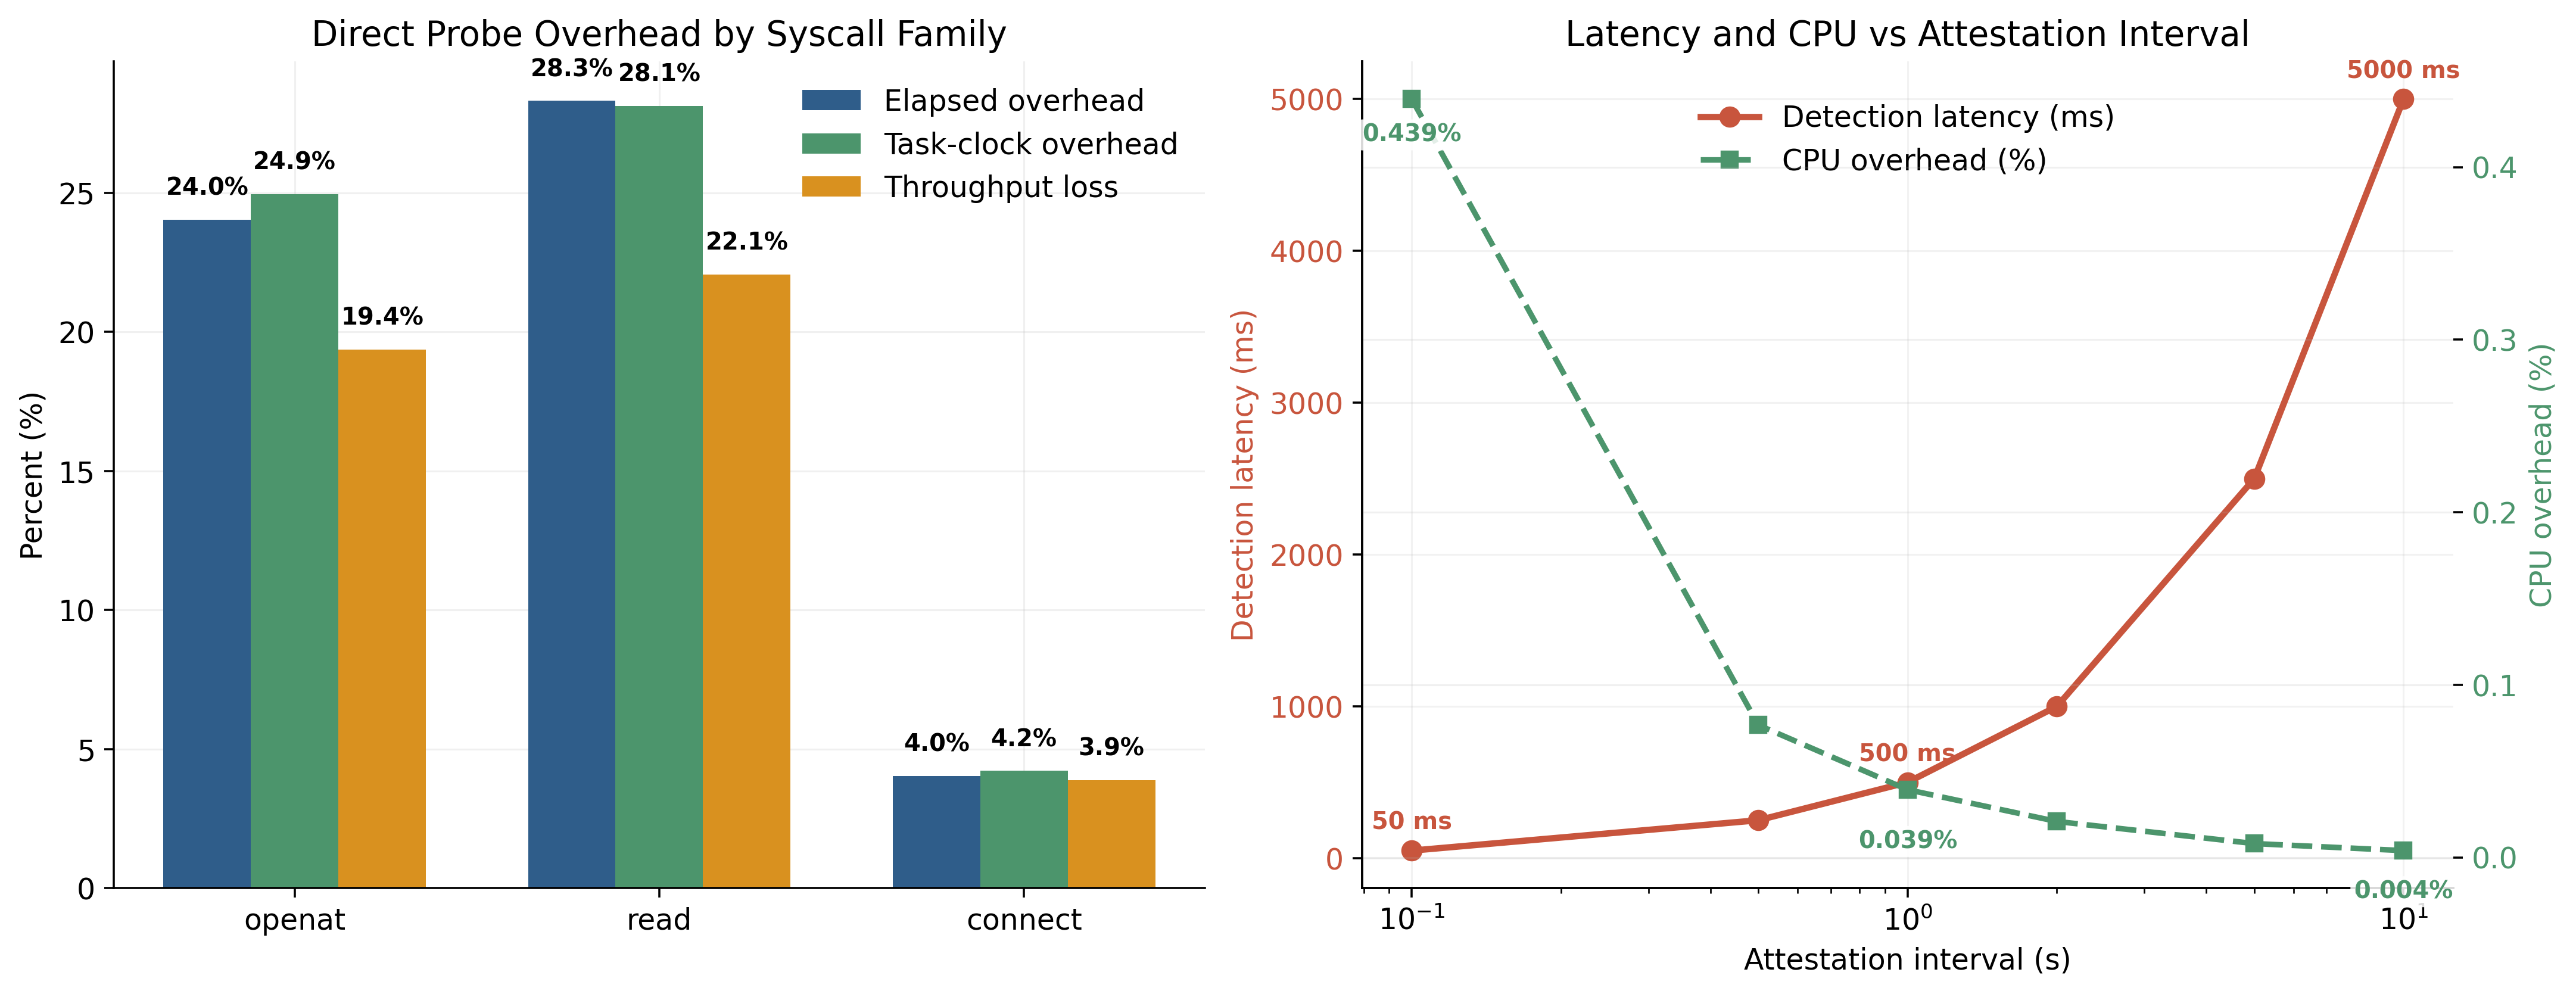
\includegraphics[width=\linewidth]{../figures/performance_overhead.png}
  \caption{Performance summary from the real measurements. Worst-case probe
  overhead is highest for file-centric syscalls, while end-to-end verifier cost
  stays below 0.44\% and falls to 0.039\% at the default 1\,s interval.}
  \label{fig:performance-overhead}
\end{figure}

We also ran a secondary simulation-based scaling study to explore regimes that
are inconvenient to measure directly on the single-node EPYC setup. As shown
in Figure~\ref{fig:scaling-sweep}, 14 of 16 tested configurations remain below
5\% overhead. In the agent-count sweep at a fixed 1\,s interval, the mixed
workload incurs 1.17\% overhead for 10 agents, 2.34\% for 50 agents, 2.12\%
for 100 agents, and 3.11\% for 500 agents. In the separate workload-type sweep
at 10 agents and 1\,s, overhead ranges from 0.30\% for compute-heavy jobs to
3.94\% for I/O-heavy jobs. We report these numbers as controlled scaling
trends rather than as deployment measurements.

\begin{figure}[t]
  \centering
  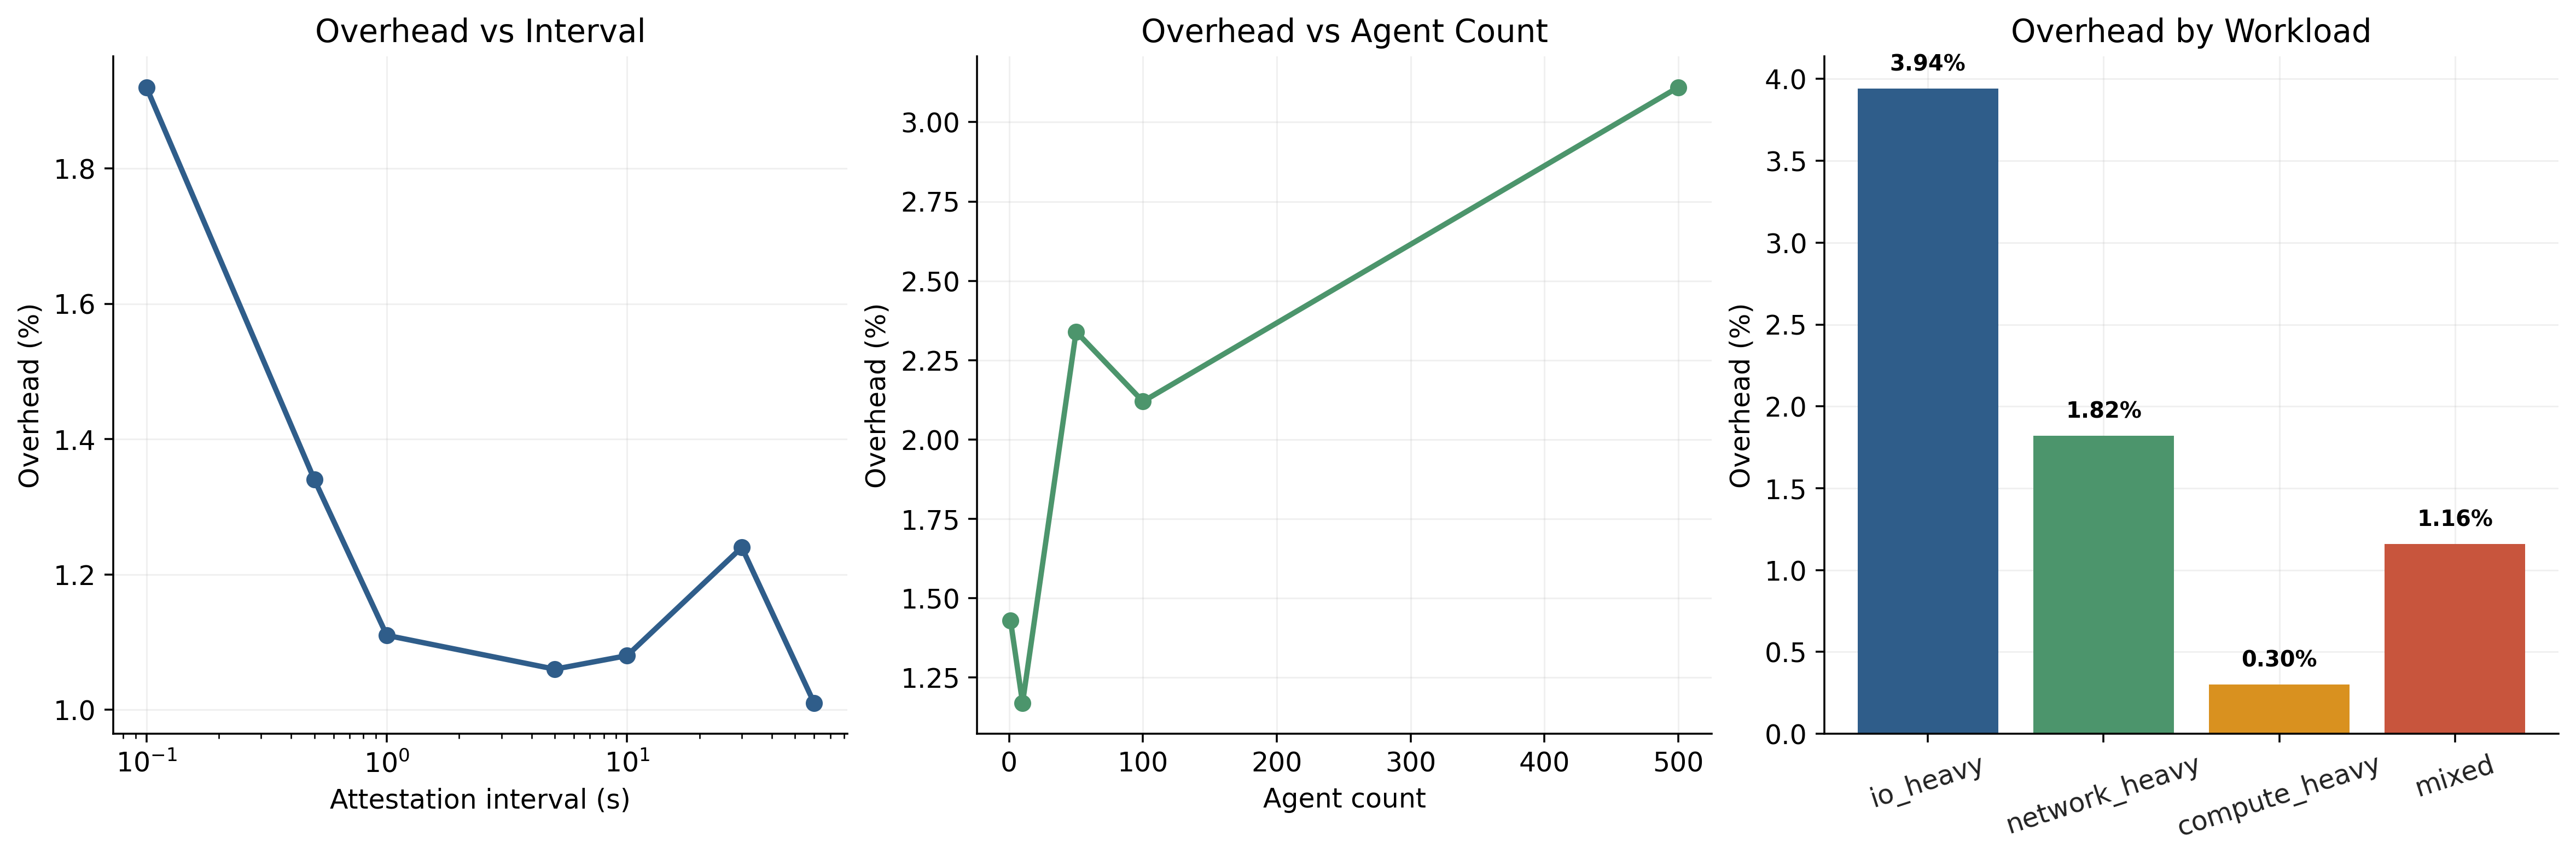
\includegraphics[width=\linewidth]{../figures/scaling_sweep.png}
  \caption{Simulation-based scaling study across attestation intervals,
  agent counts, and workload mixes. Overhead remains below 5\% in 14 of 16
  tested configurations and is dominated by I/O-heavy workloads.}
  \label{fig:scaling-sweep}
\end{figure}

\subsection{Benign Workloads}

Table~\ref{tab:false-positive-summary} summarizes the benign-workflow study.
The expanded benign-workflow suite produces no observed false positives.
Across six workflows, 42 benign actions, and 70 logged events,
\projectname~reports zero alerts. The suite is not limited to trivially clean
traces: it includes standard single-agent HPC pipelines, authorized
multi-agent collaboration, budget-edge LLM reporting, and tool-heavy
post-processing, covering both workflow breadth and benign edge cases close to
the intended policy boundary.

\begin{table*}[t]
  \caption{Benign-workflow suite used to assess false positives. Across six
  workflows, 42 benign actions and 70 logged events produce zero alerts. The
  table also summarizes which benign stress dimensions each workflow exercises.}
  \label{tab:false-positive-summary}
  \centering
  \small
  \begin{tabular}{p{4.4cm}cccp{5.4cm}c}
    \toprule
    Workflow & Agents & Actions & Logged Events & Benign Stress Exercised & Alerts \\
    \midrule
    Genomics Data Analysis & 1 & 6 & 11 & Shared-path data access; longer trace & 0 \\
    ML Training Pipeline & 1 & 7 & 12 & Tool chaining; longer trace & 0 \\
    Multi-Agent Collaboration & 2 & 8 & 14 & Shared paths; multi-agent coordination; longer trace & 0 \\
    Simulation Steering & 1 & 6 & 9 & Longer trace & 0 \\
    Budget-Edge LLM Reporting & 1 & 8 & 13 & Authorized egress near budget threshold; longer trace & 0 \\
    Tool-Heavy Climate Postprocessing & 1 & 7 & 11 & Tool chaining; longer trace & 0 \\
    \bottomrule
  \end{tabular}
\end{table*}

We emphasize the scope of this claim carefully: the result shows that no false
positives were observed on the evaluated benign suite, not that false
positives are impossible. Nevertheless, the combination of zero observed false
positives and the broadened workflow coverage suggests that declarative
behavioral constraints can remain precise enough for practical HPC agent
workloads.
